\section{matrix.cpp File Reference}
\label{matrix_8cpp}\index{matrix.cpp@{matrix.cpp}}
{\tt \#include $<$sstream$>$}\par
{\tt \#include $<$iostream$>$}\par
{\tt \#include $<$cmath$>$}\par
{\tt \#include $<$cstdlib$>$}\par
{\tt \#include $<$limits.h$>$}\par
{\tt \#include $<$sys/types.h$>$}\par
{\tt \#include \char`\"{}data\-In.h\char`\"{}}\par
{\tt \#include \char`\"{}matrix.h\char`\"{}}\par
{\tt \#include \char`\"{}utility.h\char`\"{}}\par
{\tt \#include \char`\"{}random.h\char`\"{}}\par
{\tt \#include \char`\"{}../../LASS/src/lib.h\char`\"{}}\par


Include dependency graph for matrix.cpp:\begin{figure}[H]
\begin{center}
\leavevmode
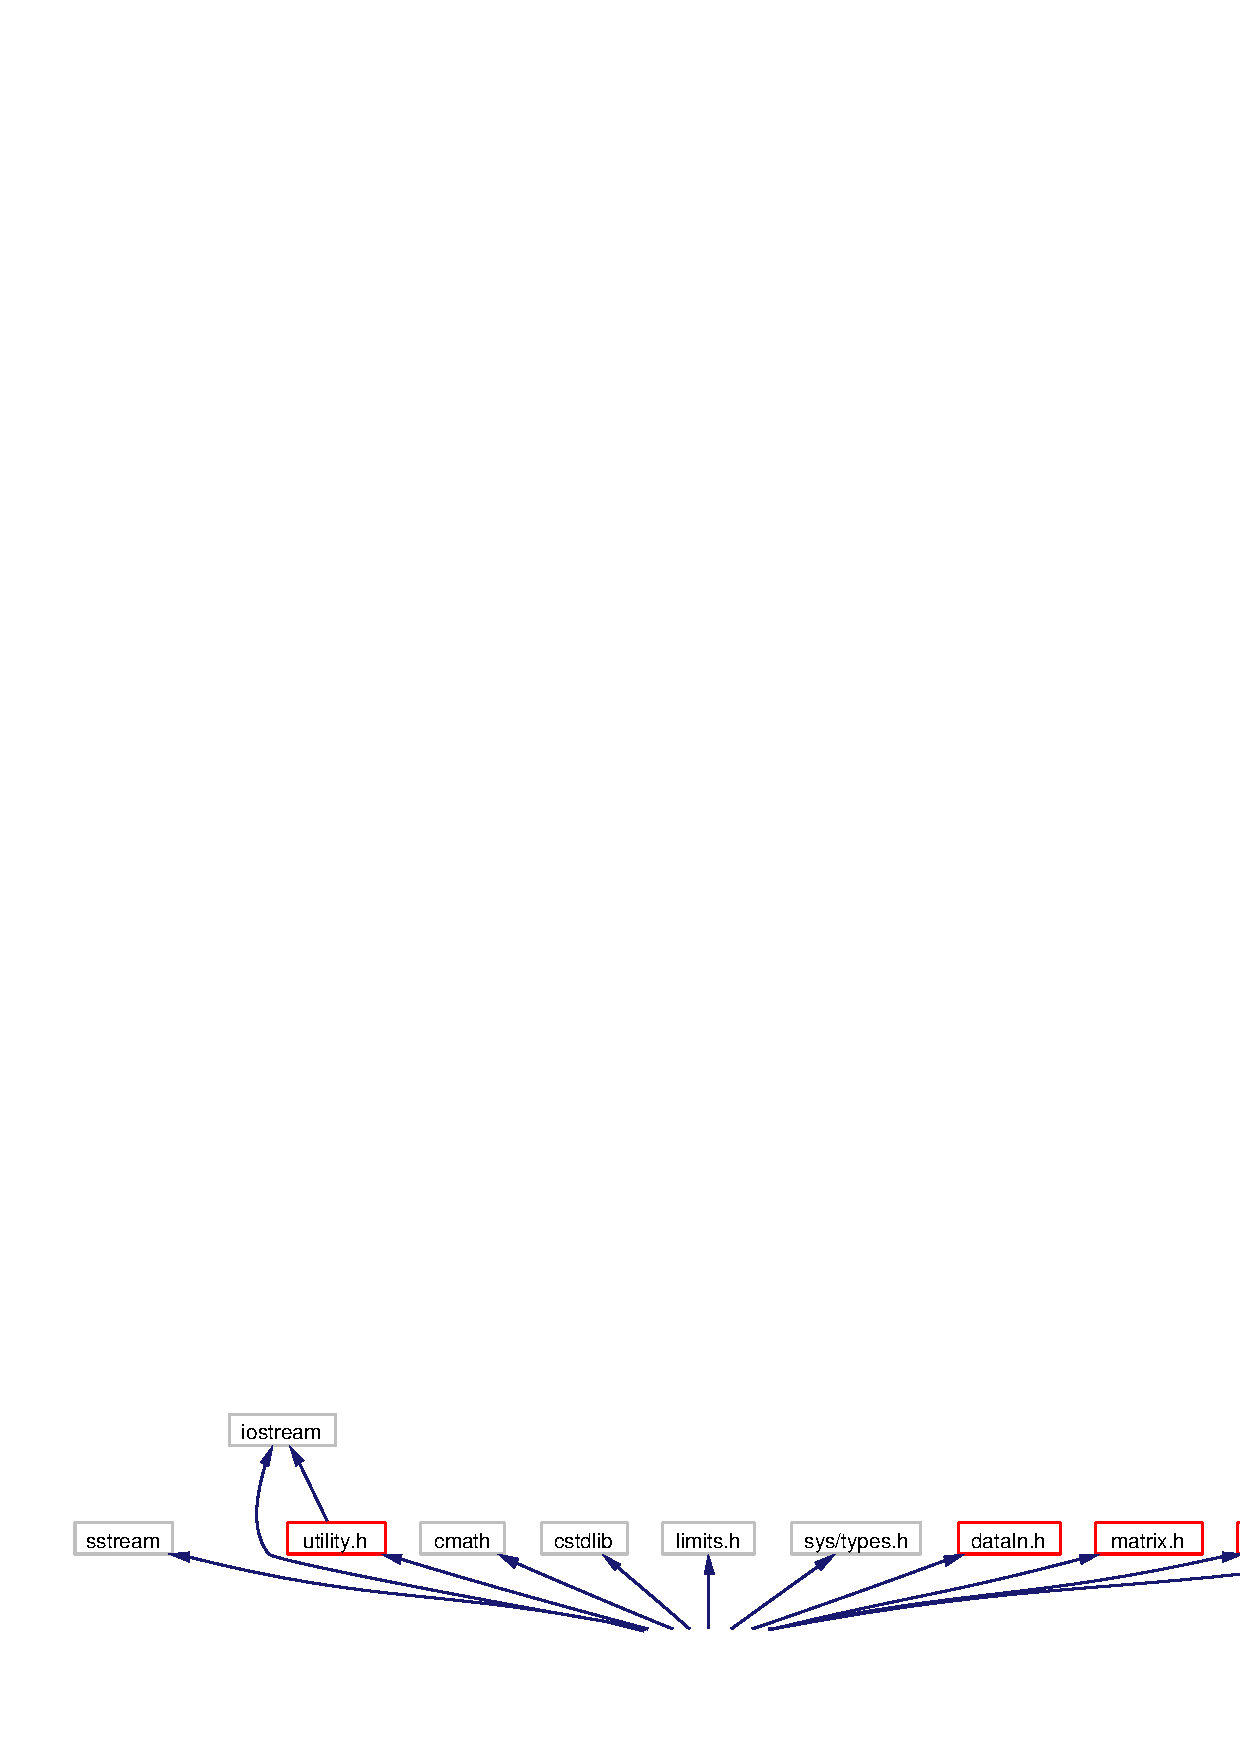
\includegraphics[width=380pt]{matrix_8cpp__incl}
\end{center}
\end{figure}
\subsection*{Functions}
\begin{CompactItemize}
\item 
ostream \& {\bf operator$<$$<$} (ostream \&s, {\bf Matrix} \&m)
\end{CompactItemize}
\subsection*{Variables}
\begin{CompactItemize}
\item 
Envelope\-Library {\bf envlib}
\end{CompactItemize}


\subsection{Function Documentation}
\index{matrix.cpp@{matrix.cpp}!operator<<@{operator$<$$<$}}
\index{operator<<@{operator$<$$<$}!matrix.cpp@{matrix.cpp}}
\subsubsection{\setlength{\rightskip}{0pt plus 5cm}ostream\& operator$<$$<$ (ostream \& {\em s}, {\bf Matrix} \& {\em m})}\label{matrix_8cpp_a1}


PUBLIC: OPERATOR$<$$<$. 

Definition at line 220 of file matrix.cpp.

References Matrix::matrix, Matrix::x, and Matrix::y.

\subsection{Variable Documentation}
\index{matrix.cpp@{matrix.cpp}!envlib@{envlib}}
\index{envlib@{envlib}!matrix.cpp@{matrix.cpp}}
\subsubsection{\setlength{\rightskip}{0pt plus 5cm}Envelope\-Library {\bf envlib}}\label{matrix_8cpp_a0}




Definition at line 43 of file matrix.cpp.